\documentclass{article}
\usepackage[a4paper, total={7in, 9.5in}]{geometry}

\setlength{\parindent}{0pt}
\setlength{\parskip}{3pt plus 1pt}


\usepackage{graphicx} % Required for inserting images

\usepackage[most]{tcolorbox}
\usepackage[export]{adjustbox}
\usepackage{lipsum}

%%%% for coding %%%%
\usepackage{listings}
\usepackage{xcolor}

\usepackage[default]{sourcesanspro} 

\usepackage[style=nature]{biblatex}
\AtBeginBibliography{\footnotesize\vspace{-8pt}}

\bibliography{references}

\definecolor{codegreen}{rgb}{0,0.6,0}
\definecolor{codegray}{rgb}{0.5,0.5,0.5}
\definecolor{codepurple}{rgb}{0.58,0,0.82}
\definecolor{backcolour}{rgb}{0.97, 0.97, 1.0}

\lstdefinestyle{mystyle}{
    backgroundcolor=\color{backcolour},   
    commentstyle=\color{codegreen},
    keywordstyle=\color{magenta},
    numberstyle=\tiny\color{codegray},
    stringstyle=\color{codepurple},
    basicstyle=\ttfamily\footnotesize,
    breakatwhitespace=false,         
    breaklines=true,                 
    captionpos=b,                    
    keepspaces=true,                 
    numbers=left,                    
    numbersep=5pt,                  
    showspaces=false,                
    showstringspaces=false,
    showtabs=false,                  
    tabsize=2
}

\lstset{style=mystyle}

\newcommand{\question}[4]{

\textbf{#1} %question \\
\begin{itemize}
\item[$\circ$] #2
\item[$\circ$] #3
%\item[$\circ$] #4
\end{itemize}

}

\newtcolorbox{mybox}[2][]{%
  enhanced,colback=white,colframe=black,coltitle=black,
  sharp corners,boxrule=0.4pt,
  fonttitle=\itshape,
  attach boxed title to top left={yshift=-0.3\baselineskip-0.4pt,xshift=2mm},
  boxed title style={tile,size=minimal,left=0.5mm,right=0.5mm,
    colback=white,before upper=\strut},
  title=#2,#1
}

\renewcommand{\sfdefault}{phv}
\renewcommand{\rmdefault}{ptm}
\renewcommand{\ttdefault}{pcr}




\begin{document}

\begin{center}
\textbf{ \Large Why you never should and certainly never have to use spreadsheets}\\
{Clara Kofler (originally written for the RV newspaper \emph{Distribution})}
\end{center}

For almost no experimentalist a week goes by without data analysis. This is no one's favorite job but it has to be done, and it has to be done well; otherwise, what is the point of recording the data at all?

There are obviously many means to that end - all roads lead to Rome. However, some roads will be more painful than others, some roads will lead to more then 20\% of papers featuring gene names containing wrong data \cite{Lewis2021} and some roads will lead to international humiliation of the Austrian government \cite{standard-excel}.

To ensure you do not have to go down these roads (and also because it is just more convenient in every way), here a short tutorial on using python to do your data analysis. 

\dotfill\\
%\setlength{\columnsep}{-3cm}

\textbf{\large Setting up your system:}\\
The easiest way to do data analysis with python is by using Jupyter, a web interface for interactive computing. We will use conda to set this up. If you already have a running conda and jupyterlab, please skip the following steps.\\

\textbf{Installing Miniconda}\\
If you already have Miniconda or another version of conda, please skip this paragraph.

To install Miniconda, follow the steps for your operating system on their website: \url{https://docs.anaconda.com/miniconda/miniconda-install/}

After doing this, Windows users should find an Anaconda Prompt application on their system, opening up a command line window. Linux and Mac OS users should see a new (base) prefix in their terminal after restarting it.  \\

\noindent
\begin{minipage}{.65\textwidth}

\textbf{Installing Jupyterlab in a new environment}\\
Please follow the following commands in your conda prompt/terminal to set up a new virtual environment and install the needed packages: 

\begin{lstlisting}[language=bash, numbers=none]   
    $ conda create -n data-analysis python 
    $ conda activate data-analysis\end{lstlisting}

This should create a new environment named \emph{data-analysis} and activate it. You should see the (base) change to (data-analysis) as you change environment. 
You can deactivate the environment with \texttt{conda deactivate}, and activate it again any time.

Then install the packages we need in this environment:

\begin{lstlisting}[language=bash, numbers=none]   
    $ conda install -c conda-forge jupyterlab
    $ conda install -c anaconda git
    $ conda install -c conda-forge pandas
    $ conda install scipy matplotlib tabulate
\end{lstlisting}

\vspace{3pt}
\textbf{Cloning example data and notebook}\\
I have created a starting notebook and shared it on github, please clone it to a folder of your choice using:

\begin{lstlisting}[language=bash, numbers=none]   
    $ git clone https://github.com/kofcla/data-analysis-tutorial.git
\end{lstlisting}

\textbf{Now open jupyter} by typing 

\begin{lstlisting}[language=bash, numbers=none]   
    $ jupyter lab 
\end{lstlisting}

(you might need to copy the link into your browser). 

There, open \textbf{data-analysis-tutorial.jpynb}. 

\end{minipage}% This must go next to `\end{minipage}`
\hspace{.01\textwidth}\begin{minipage}{.35\textwidth}

  \centering
  
\includegraphics[width=.7\linewidth]{figures/chatgpt-python.png}\\
  \textcolor{gray}{\tiny Image by ChatGPT}

  \begin{mybox}{Useful bash commands}

        \centering
        \begin{tabular}{l|l}
            ls & list contents \\
            cd <dir>  & move to <dir> \\ 
            mkdir <dir> & create new folder \\
            rm <file> & delete <file> \\
            mv <thg> <plce> & move things \\
            cp <thg> <plce> & copy things \\
            pwd & where am I?
        \end{tabular}

  \end{mybox}

\end{minipage}

%\vspace{.5cm}

%\textbf{So, lets get to it! Run jupyterlab and open the notebook data-analysis-example.jpynb!}

%\setlength{\columnsep}{3mm}

%\vspace{-10pt}

\nocite{reference}
\printbibliography[keyword={data-analysis}, title=\normalsize References]


 \newpage

\begin{center}

\textbf{ \Large The basics of data visualization and analysis}

\end{center}

\textbf{How to use this page:} The bread and butter of learning programming is to try out things and play around with it. We cannot do that for you unfortunately. But here we want to help you get started. 

The example notebook \lstinline{data-analysis-example.ipynb} had examples of creating plots and doing data analysis tasks similar to what you encounter in lab courses. We provide explanations and small tasks for you. Please note that we show one way to do it, but it is by far not the only way. So, have a look through the notebook, do the tasks, play around with the code! 

The rest of this page contains examples similar to the notebook and suggestions for the packages to use for certain tasks. This should give you a quick overview of what we cover in the notebook.

\dotfill
\vspace{5pt}

\noindent
\begin{minipage}{.5\textwidth}
\textbf{\large Loading data}\\
To load your data we advise you to use \lstinline{numpy}. It is specialized for dealing with arrays, so perfect for handling numerical data. It also has a lot of math functionalities that will prove useful.

If you want to look at your data in the form of a table you should use \lstinline{pandas}. It has the so-called DataFrames that are very convenient to work with. 

\end{minipage}% This must go next to `\end{minipage}`
\hspace{.05\textwidth}\begin{minipage}{.5\textwidth}
\begin{lstlisting}[language=python, numbers=none]   
#basic example of numpy data loading
data = np.loadtxt('my_filename.csv', delimiter=',')

#reading as csv file into pandas dataframe
df = pandas.read_csv('my_filename.csv')
    
\end{lstlisting}
\end{minipage}

\vspace{5pt}
\noindent
\begin{minipage}{.5\textwidth}

\textbf{\large Creating simple plots}\\
There are a million ways to plot something in python, we decided on using \lstinline{matplotlib}. This package provides a massive amount of data visualization possibilities. Sometimes it is a bit unintuitive but it gets the job done. 

\begin{lstlisting}[language=python, numbers=none]   
#basic plotting

plt.plot(x1, y, marker='^', ls='', color='coral', label='data 1') 
plt.plot(x1, z, marker='*', ls='', color='teal', label='data 2') 

plt.xlabel('random x')
plt.ylabel('random y')
plt.title('Random things')
plt.legend()

plt.show()    
\end{lstlisting}

\end{minipage}% This must go next to `\end{minipage}`
\hspace{.05\textwidth}\begin{minipage}{.5\textwidth}
  \centering
  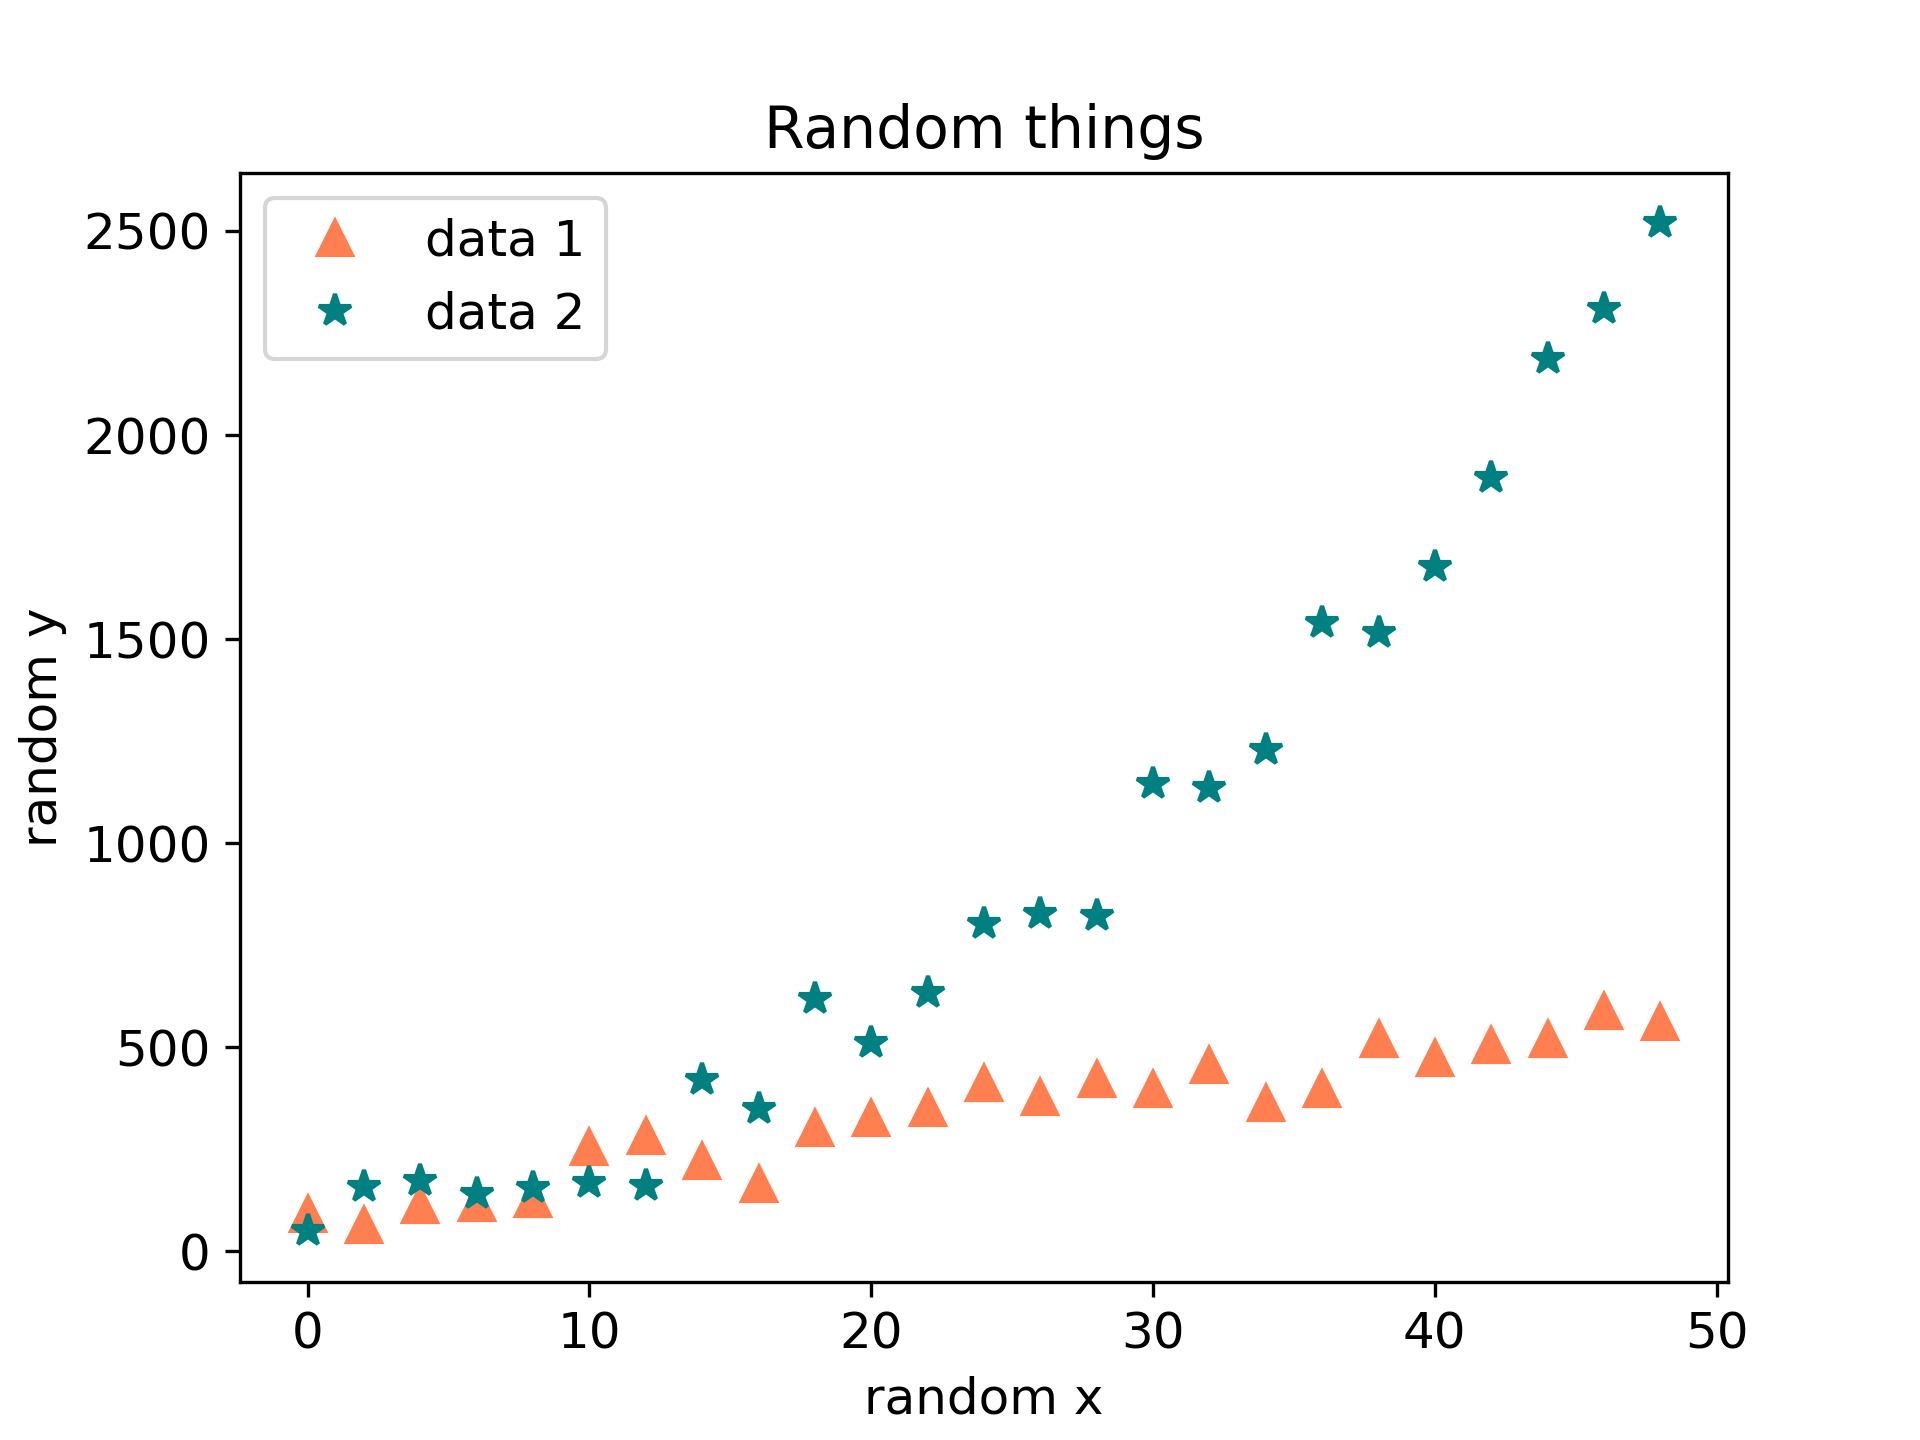
\includegraphics[width=.9\linewidth]{figures/simple-plot.png}\\

\end{minipage}

\noindent
\begin{minipage}{.5\textwidth}
\textbf{\large Fitting data}\\
For data fitting, we recommend \lstinline{scipy}. This package contains many analysis tools, including an optimization module that offers different functions for data fits. Here the important thing is to provide proper starting values, otherwise, your fits will not converge. For curve fitting \lstinline{scipy.optimize.curve_fit} works well.

Pro tip: If you need to use scientific constants you can import them from \lstinline{scipy.constants}.

\vspace{5pt}

\textbf{\large Image processing}\\
For image processing you can use the \lstinline{scipy.ndimage}. Also \lstinline{numpy} offers certain helpful functionalities. Depending on your specific task there might already be some more specified python package. You can install it in your environment like we did on the previous page. 

\vspace{5pt}

\textbf{\large Exporting LaTex tables}\\
The package \lstinline{tabulate} is amazing for creating simple tables. With the command \lstinline{tabulate(table, headers, tablefmt="latex")} you can create a table to copy into your LaTex document. 


\end{minipage}% This must go next to `\end{minipage}`
\hspace{.05\textwidth}\begin{minipage}{.5\textwidth}
\begin{mybox}{Tips for nice figures:}
\begin{enumerate}
    \item Before you start, think about the story of the figure. What do you want to show? Choose the data accordingly.\vspace{-8pt}
    \item Try to manipulate the raw data as little as possible. If you have to, make sure to document it properly and communicate it transparently. \vspace{-8pt}
    \item Think about what type of plot best presents your argument. \vspace{-8pt}
    \item Take a pen and sketch the figure before you start plotting.\vspace{-8pt}
    \item You want to avoid rescaling. So choose your font and object sizes wisely.\vspace{-8pt}
    \item Make sure to save the images as vector graphics (SVG or PDF) and with a high enough DPI value (e.g. 300).\vspace{-8pt}
    \item Check if the saved figure looks like you want it to.\vspace{-8pt}
    \item If you need to make larger plots containing many sub figures consider assembling them in a vector graphics program like \emph{Inkscape}.
\end{enumerate}
    
\end{mybox}

\end{minipage}


\end{document}
